\documentclass[12pt,a4paper]{article}

\usepackage{geometry}
\geometry{a4paper, margin=2cm}

%======================================================================================
% Includes/packages

\usepackage{graphicx}
\usepackage{amsmath}
\usepackage{listings}
\usepackage{float}
\usepackage{comment}
% Long equations
\usepackage{breqn}
\usepackage{amsmath}
% Sub figures
\usepackage{caption}
\usepackage{subcaption}
\usepackage{tabularx} % Include this in your preamble
% Real number R symbol
\usepackage{amssymb}

%======================================================================================

% atan2
\DeclareMathOperator{\atantwo}{atan2}

% norm
\newcommand\norm[1]{\left\lVert#1\right\rVert}

%======================================================================================

% Create document

\title{ELA408 - Lab 1: Navigating a Maze with a Differential Drive Robot}
\author{Carl Larsson, Pontus Svensson}
\date{\today}

\begin{document}

\maketitle

% Include sections
%\begin{abstract}
%======================================================================================

%======================================================================================
\end{abstract}


%======================================================================================
\begin{comment}
    
\end{comment}
%======================================================================================
\section{Introduction}
%======================================================================================

This paper covers Lab 1, the development of a differential drive model robot wrapped inside of a unicycle model with go to goal, avoid obstacle and wall follow behavior.


% Differential drive
% Discuss the differential drive model and its equations.
% Importance
Most robots suffer the control constraints of having two motorized wheels, differential drive model is a control model for robots with two motorized wheels. 
% Workings
The differential drive model works in terms of desired scalar left and right wheel velocities, however this is not ideal since it is unintuitive to control. Preferably, the desired linear and angular velocity would be specified, not the desired left and right wheel velocities.
For the differential drive model, with scalar wheel velocities $v_l$ and $v_r$, and wheel parameters radius $r$ and wheel base $l$, the $\dot{x}$, $\dot{y}$ and $\dot{\theta}$ can be acquired according to\:\eqref{eq:differential_drive_model}\:\cite{carlenerikssonLectureKinematicsBehavioral2024}.
\begin{equation}
    \label{eq:differential_drive_model}
    \begin{cases}
    \dot{x} = \frac{r}{2} (v_r + v_l) \cos{\theta} \\
    \dot{y} = \frac{r}{2} (v_r + v_l) \sin{\theta} \\
    \dot{\theta} = \frac{r}{l} (v_r - v_l)
    \end{cases}
\end{equation}


% Unicle model
% Describe the unicycle model and present its theoretical equations.
% Importance
To work with desired linear and angular velocities the help of the unicycle model can be employed, simply wrapping the underlying system constraints, which are part of the differential drive model, inside of the unicycle model.
The unicycle model is much easier to work with since it is the easier way to control and model robots, simply specifying the desired movement of the robot rather than individual wheel velocities.
% Workings
For the unicycle model, with scalar inputs linear velocity $v$ and angular velocity $\omega$, the $\dot{x}$, $\dot{y}$ and $\dot{\theta}$ can be acquired according to\:\eqref{eq:unicycle_model}\:\cite{carlenerikssonLectureKinematicsBehavioral2024}.
\begin{align}
    \label{eq:unicycle_model}
    \begin{cases}
    \dot{x} = v \cos{\theta} \\
    \dot{y} = v \sin{\theta} \\
    \dot{\theta} = \omega
    \end{cases}
\end{align}


% Explain how the unicycle model can be designed using the differential drive model.
By equating\:\eqref{eq:differential_drive_model} and\:\eqref{eq:unicycle_model}, the connection between unicycle model and differential drive model can be obtained, see\:\eqref{eq:left_uni_differential} and\:\eqref{eq:right_uni_differential}\:\cite{carlenerikssonLectureKinematicsBehavioral2024}.
\begin{dmath}
    \label{eq:left_uni_differential}
    v_l = \frac{2 v - \omega l}{2 r}
\end{dmath}

\begin{dmath}
    \label{eq:right_uni_differential}
    v_r = \frac{2 v + \omega l}{2 r}
\end{dmath}
When using\:\eqref{eq:left_uni_differential} and\:\eqref{eq:right_uni_differential} in\:\eqref{eq:differential_drive_model}, the input and output remains the same, with the intuitive input of the unicycle model, resulting in essentially wrapping or encapsulating the differential drive model inside of the unicycle model.

%======================================================================================


%======================================================================================
\begin{comment}
    % Provide an introduction to the concepts of the unicycle model, differential drive model, and the importance of these models in robotic navigation.
\end{comment}
%======================================================================================
%\section{Theoretical Background}
%======================================================================================

\subsection{Unicycle Model}
% Describe the unicycle model and present its theoretical equations.

For the unicycle model, with scalar linear velocity $v$ and angular velocity $\omega$, the $\dot{x}$, $\dot{y}$ and $\dot{\theta}$ can be acquired according to\:\eqref{eq:unicycle_model}\:\cite{carlenerikssonLectureKinematicsBehavioral2024}.

\begin{align}
    \label{eq:unicycle_model}
    \begin{cases}
    \dot{x} = v \cos{\theta} \\
    \dot{y} = v \sin{\theta} \\
    \dot{\theta} = \omega
    \end{cases}
\end{align}

%======================================================================================

\subsection{Differential Drive Model}
% Discuss the differential drive model and its equations.

For the differential drive model, with scalar wheel velocities $v_l$ and $v_r$, and wheel parameters radius $r$ and wheel base $l$, the $\dot{x}$, $\dot{y}$ and $\dot{\theta}$ can be acquired according to\:\eqref{eq:differential_drive_model}\:\cite{carlenerikssonLectureKinematicsBehavioral2024}.

\begin{align}
    \label{eq:differential_drive_model}
    \begin{cases}
    \dot{x} = \frac{r}{2} (v_r + v_l) \cos{\theta} \\
    \dot{y} = \frac{r}{2} (v_r + v_l) \sin{\theta} \\
    \dot{\theta} = \frac{r}{l} (v_r - v_l)
    \end{cases}
\end{align}

%======================================================================================

\subsection{Connection Between Models}
% Explain how the unicycle model can be designed using the differential drive model.

By equating\:\eqref{eq:unicycle_model} and\:\eqref{eq:differential_drive_model}, the connection between unicycle model and differential drive model can be obtained, see\:\eqref{eq:left_uni_differential} and\:\eqref{eq:right_uni_differential}\:\cite{carlenerikssonLectureKinematicsBehavioral2024}.

\begin{dmath}
    \label{eq:left_uni_differential}
    v_l = \frac{2 v - \omega l}{2 r}
\end{dmath}

\begin{dmath}
    \label{eq:right_uni_differential}
    v_r = \frac{2 v + \omega l}{2 r}
\end{dmath}

When using\:\eqref{eq:left_uni_differential} and\:\eqref{eq:right_uni_differential} in\:\eqref{eq:differential_drive_model}, the input and output remains the same, with the intuitive input of the unicycle model, resulting in essentially wrapping or encapsulating the differential drive model inside of the unicycle model.

%======================================================================================


%======================================================================================
\begin{comment}
    
\end{comment}
%======================================================================================
\section{Method}
%======================================================================================

The entire system was created and simulated in Matlab R2023b, Simulink and Stateflow using the model and maze provided by the assignment.

%======================================================================================

\subsection{Differential drive model}
% Detail how you expanded the unicycle model to include the differential drive robot model.

The model provided was expanded to work based on a differential drive model. This was achieved by letting the inputs remain as linear velocity $v$ and angular velocity $\omega$. However the method used to obtain $\dot{x}$, $\dot{y}$ and $\dot{\theta}$ was no longer\:\eqref{eq:unicycle_model}. Instead\:\eqref{eq:left_uni_differential} and\:\eqref{eq:right_uni_differential} was used in combination with\:\eqref{eq:differential_drive_model}. With this, the input and output remained the same, resulting in modeling the system as a whole as a unicycle model, but with the internal workings of a differential drive model.

%======================================================================================

\subsection{Parameters}
% Detail parameters

The system parameters were:
\begin{itemize}
    \item Wheel radius: $r = 0.1$
    \item Wheel base: $l = 0.5$
    \item Follow wall behavior threshold: $\Delta_1 = 1$
    \item Avoid obstacle behavior threshold: $\Delta_2 = 0.5$
    \item Constant velocity: $v = 0.1$
    \item Proportional gain: $P = 10$
    \item Tolerance distance to goal: $\epsilon = 0.01$
    \item Simulation time: $t_s = 1100$
\end{itemize}
Note that parameters included in the model provided are not covered, this includes e.g. start and goal position.
As can be seen from the parameters, only a simple proportional controller was used for control, no $I$ or $D$ part.
All parameters was specified in a initialization Matlab script.

%======================================================================================

\subsection{Designing Behaviors}
% Discuss how you designed the required behaviors:

The different behaviors of the system are detailed in this section, go to goal (GTG), avoid obstacle (AO), follow wall (FW) clockwise (c) and counter clockwise (cc).
A complete version of the go to goal behavior was already present in the provided model, the only development made to this consisted of the transitions from this behavior to others. See Fig.\:\eqref{fig:behavior_transitions} for all transitions between behaviors. The transitions was implemented in Stateflow.
\begin{figure}
    \centering
    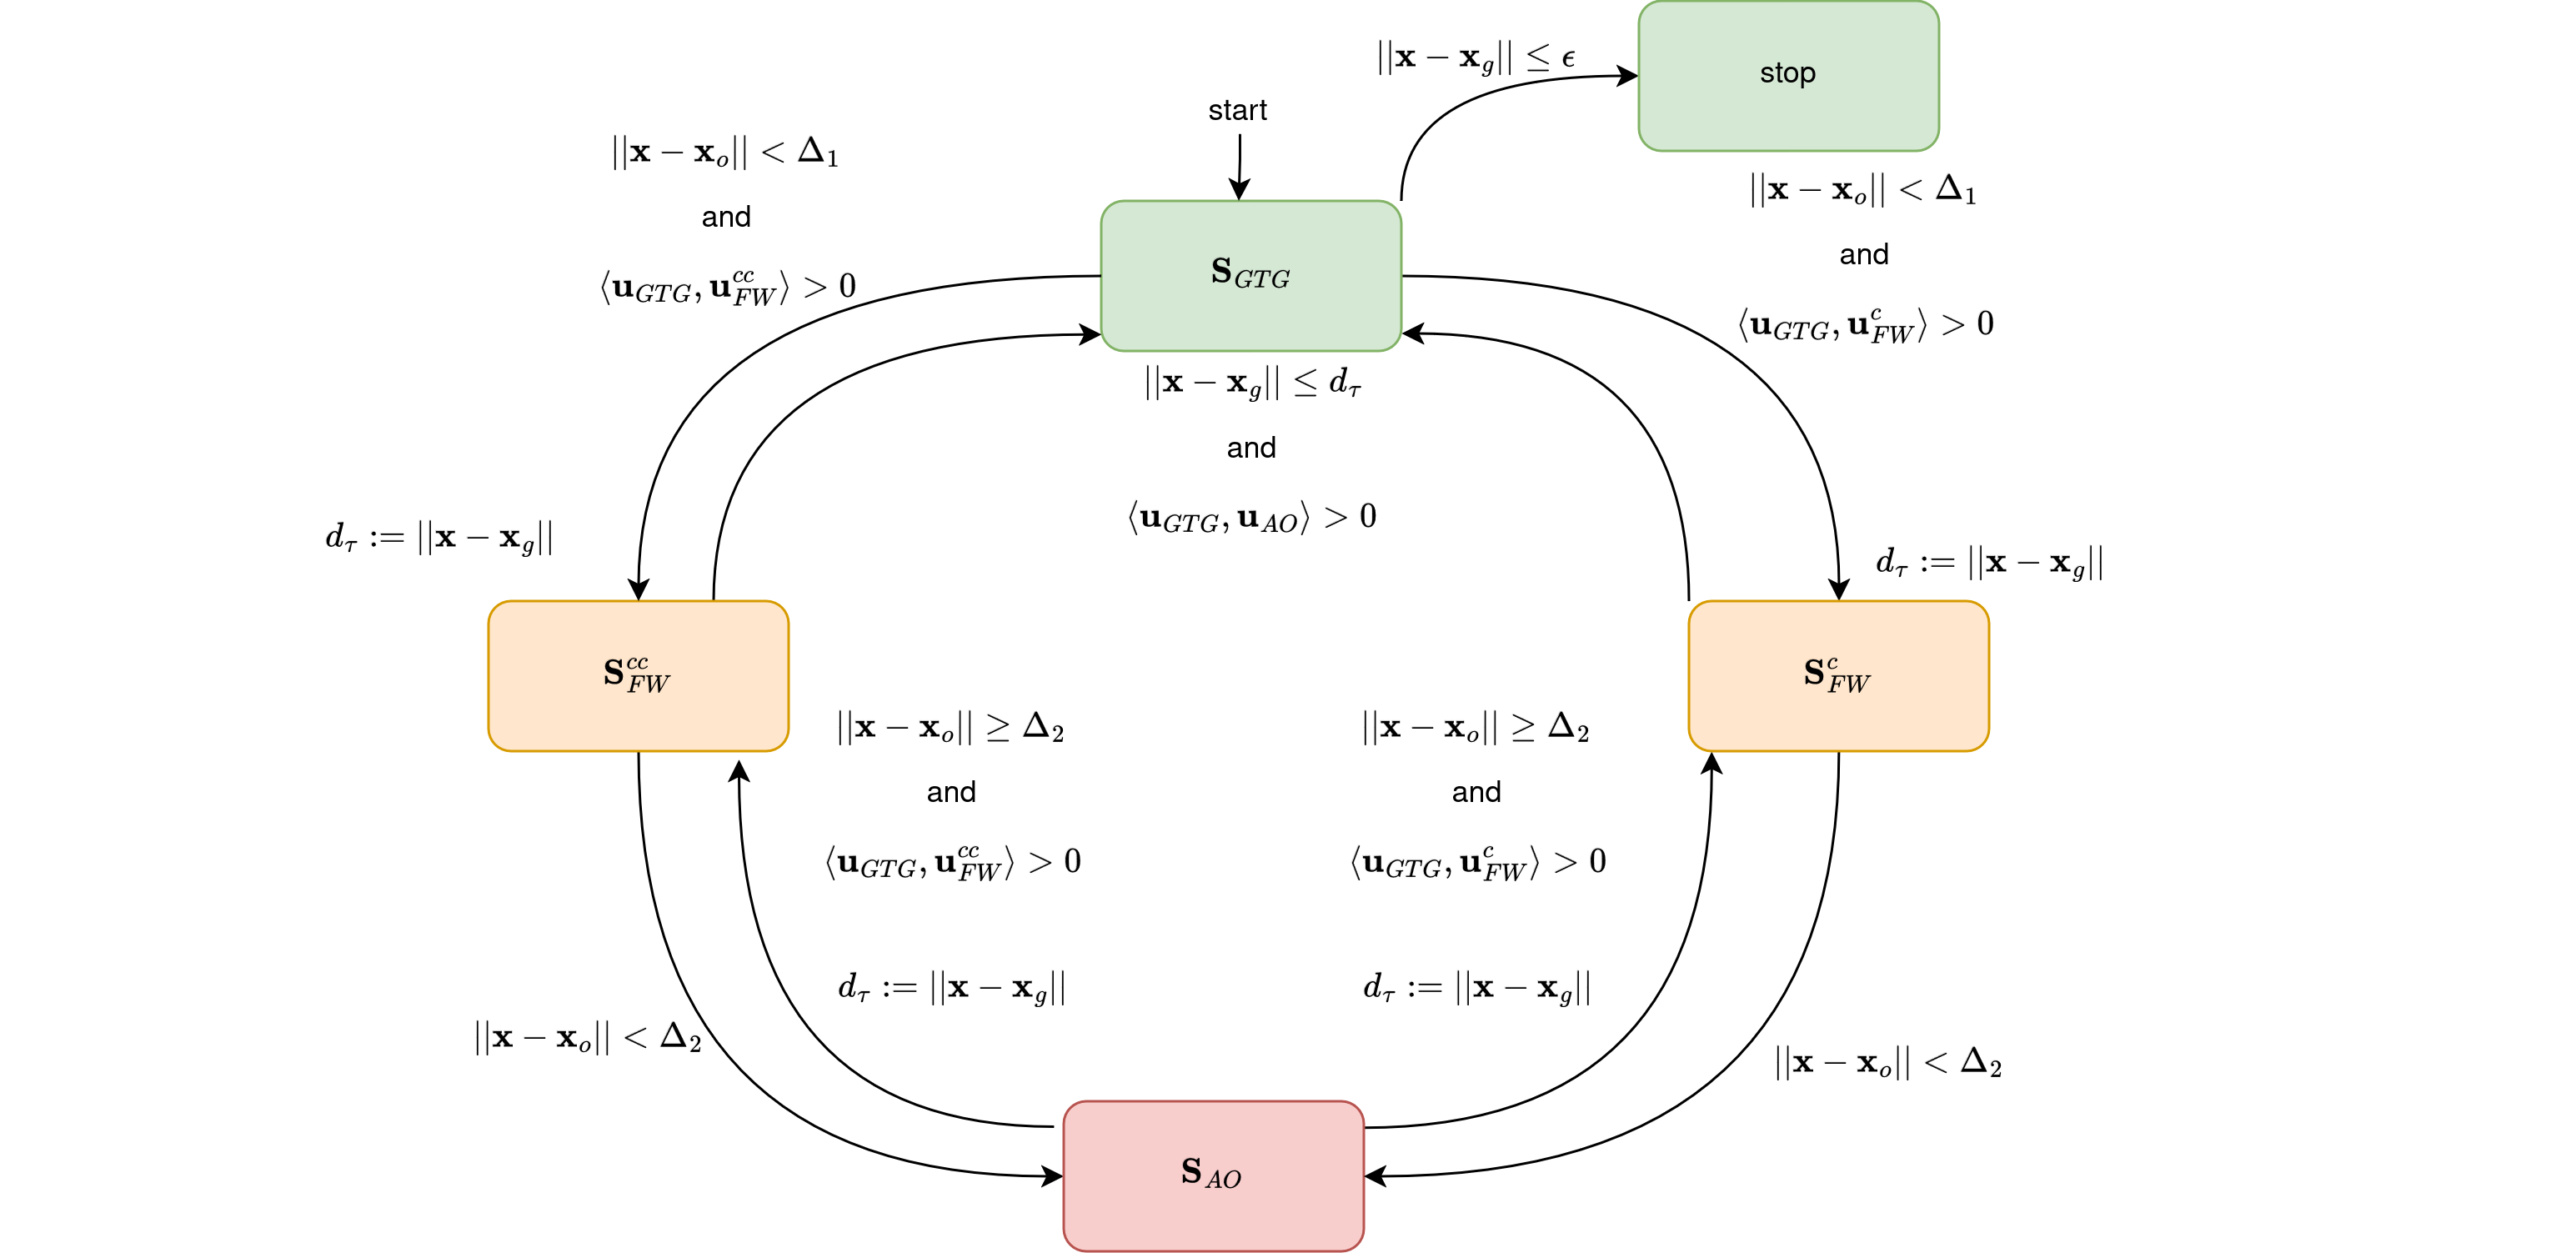
\includegraphics[width=\columnwidth]{images/flowchat_lab1.png}
    \caption{All possible transitions between every behavior.}
    \label{fig:behavior_transitions}
\end{figure}




\subsubsection{Calculations}
All distances were calculated using Euclidean distance, see\:\eqref{eq:euclidean_distance} for 2-D vectors in Euclidean xy-plane, the formula can be further expanded to include vectors of any dimension.
\begin{equation}
    \label{eq:euclidean_distance}
    d = \norm{ \mathbf{x} - \mathbf{x}_p } = \sqrt{(x-x_p)^2 + (y-y_p)^2}
\end{equation}
where $\mathbf{x} = [x,y]^T$ is the robots position and $\mathbf{x}_p = [x_p, y_p]^T$ is an arbitrary target point.
Note that $\mathbf{x}$ refers to a vector (specifically the position vector of the robot), while $x$ refers to a scalar, the x coordinate in Euclidean space.

$d_\tau$ is the distance from the robot to the goal at time $t = \tau$, see\:\eqref{eq:d_tau}.
\begin{equation}
    \label{eq:d_tau}
    d_\tau := \norm{ \mathbf{x}(\tau) - \mathbf{x}_g } = \sqrt{(x(\tau)-x_g)^2 + (y(\tau)-y_g)^2}
\end{equation}
where the subscript $g$ refers to goal.

$\langle *, * \rangle$ refers to the dot product between two vectors, sometime also written as $*\cdot*$. The dot product describes if the angle between two vectors is less than $\frac{\pi}{2}$ ($\langle *, * \rangle > 0$), equal to $\frac{\pi}{2}$ ($\langle *, * \rangle = 0$), or more than $\frac{\pi}{2}$ ($\langle *, * \rangle < 0$). Three different dot products are necessary for this system, see\:\eqref{eq:angle_goal_ao},\:\eqref{eq:angle_goal_c} and\:\eqref{eq:angle_goal_cc}\:\cite{carlenerikssonLectureKinematicsBehavioral2024}. 
\begin{dmath}
    \label{eq:angle_goal_ao}
    \langle \mathbf{u}_{GTG} , \mathbf{u}_{AO} \rangle
\end{dmath}
\begin{dmath}
    \label{eq:angle_goal_c}
    \langle \mathbf{u}_{GTG} , \mathbf{u}_{FW}^{c} \rangle
\end{dmath}
\begin{dmath}
    \label{eq:angle_goal_cc}
    \langle \mathbf{u}_{GTG} , \mathbf{u}_{FW}^{cc} \rangle
\end{dmath}
(Note that standard dot product in Euclidean space is commutative.)
Where $\mathbf{u}_{GTG}$, $\mathbf{u}_{AO}$, $\mathbf{u}_{FW}^{c}$ and $\mathbf{u}_{FW}^{cc}$ can be obtained according to\:\eqref{eq:u_gtg},\:\eqref{eq:u_ao},\:\eqref{eq:u_fw_c} and\:\eqref{eq:u_fw_cc}\:\cite{carlenerikssonLectureKinematicsBehavioral2024}.
\begin{dmath}
    \label{eq:u_gtg}
    \mathbf{u}_{GTG} = \mathbf{x}_g - \mathbf{x}
\end{dmath}
\begin{dmath}
    \label{eq:u_ao}
    \mathbf{u}_{AO} = \mathbf{x} - \mathbf{x}_o
\end{dmath}
\begin{dmath}
    \label{eq:u_fw_c}
    \mathbf{u}_{FW}^{c} = \mathbf{R}_{\text{z}}(-\pi/2) \mathbf{u}_{AO}
\end{dmath}
\begin{dmath}
    \label{eq:u_fw_cc}
    \mathbf{u}_{FW}^{cc} = \mathbf{R}_{\text{z}}(\pi/2) \mathbf{u}_{AO}
\end{dmath}
Note that in this specific case where all the vectors are in the 2-D Euclidean xy-plane, and thus of dimension 2, then $\mathbf{R}_{\text{z}}(\phi) \in \mathbb{R}^{2\times2}$ (note that the $\text{z}$ could be omitted but is included for clarity).

All the angles in the system were constrained to the interval $[-\pi, \pi]$ using the $\atantwo(y,x)$ function.




\subsubsection{Transitions}
There are multiple transitions between each behavior, all described in Fig.\:\ref{fig:behavior_transitions}. The transitions will also be described here for additional clarity. The transitions will be presented in terms of equations, if all the equation conditions hold, then the transition is executed.

% GTG
Go to goal had three possible transitions: stop simulation (goal reached), follow wall clockwise and follow wall counter clockwise.
Transition from go to goal to stop simulation was executed if\:\eqref{eq:gtg_to_ss} was satisfied.
\begin{equation}
    \label{eq:gtg_to_ss}
    \norm{ \mathbf{x} - \mathbf{x}_g } \le \epsilon
\end{equation}
Transition from go to goal to follow wall clockwise was executed if\:\eqref{eq:gtg_to_fw_c} was satisfied. At the particular time instant $\tau$ at which this transition was executed, $d_{\tau}$\:\eqref{eq:d_tau} was saved.
\begin{equation}
    \label{eq:gtg_to_fw_c}
    \begin{cases}
         \norm{ \mathbf{x} - \mathbf{x}_o } < \Delta_1 \\
         \langle \mathbf{u}_{GTG} , \mathbf{u}_{FW}^{c} \rangle > 0
    \end{cases}
\end{equation}
Transition from go to goal to follow wall counter clockwise was executed if\:\eqref{eq:gtg_to_fw_cc} was satisfied. At the particular time instant $\tau$ at which this transition was executed, $d_{\tau}$\:\eqref{eq:d_tau} was saved.
\begin{equation}
    \label{eq:gtg_to_fw_cc}
    \begin{cases}
         \norm{ \mathbf{x} - \mathbf{x}_o } < \Delta_1 \\
         \langle \mathbf{u}_{GTG} , \mathbf{u}_{FW}^{cc} \rangle > 0
    \end{cases}
\end{equation}

% FW C
Follow wall clockwise had two possible transitions: go to goal and avoid obstacles.
Transition from follow wall clockwise to go to goal was executed if\:\eqref{eq:fw_c_to_gtg} was satisfied.
\begin{equation}
    \label{eq:fw_c_to_gtg}
    \begin{cases}
        \norm{ \mathbf{x} - \mathbf{x}_g } \le d_{\tau} \\
        \langle \mathbf{u}_{GTG} , \mathbf{u}_{AO} \rangle > 0
    \end{cases}
\end{equation}
Transition from follow wall clockwise to avoid obstacle was executed if\:\eqref{eq:fw_c_to_ao} was satisfied.
\begin{equation}
    \label{eq:fw_c_to_ao}
    \begin{cases}
        \norm{ \mathbf{x} - \mathbf{x}_o } < \Delta_2
    \end{cases}
\end{equation}

% FW CC
Follow wall counter clockwise had two possible transitions: go to goal and avoid obstacles. Note that these transition conditions are identical to the previous two for follow wall clockwise.
Transition from follow wall counter clockwise to go to goal was executed if\:\eqref{eq:fw_cc_to_gtg} was satisfied.
\begin{equation}
    \label{eq:fw_cc_to_gtg}
    \begin{cases}
        \norm{ \mathbf{x} - \mathbf{x}_g } \le d_{\tau} \\
        \langle \mathbf{u}_{GTG} , \mathbf{u}_{AO} \rangle > 0
    \end{cases}
\end{equation}
Transition from follow wall counter clockwise to avoid obstacle was executed if\:\eqref{eq:fw_cc_to_ao} was satisfied.
\begin{equation}
    \label{eq:fw_cc_to_ao}
    \begin{cases}
        \norm{ \mathbf{x} - \mathbf{x}_o } < \Delta_2
    \end{cases}
\end{equation}

% AO
Avoid obstacles had two possible transitions: follow wall clockwise and follow wall counter clockwise.
Transition from avoid obstacles to follow wall clockwise was executed if\:\eqref{eq:ao_to_fw_c} was satisfied. At the particular time instant $\tau$ at which this transition was executed, $d_{\tau}$\:\eqref{eq:d_tau} was saved.
\begin{equation}
    \label{eq:ao_to_fw_c}
    \begin{cases}
        \norm{ \mathbf{x} - \mathbf{x}_o } \ge \Delta_2 \\
        \langle \mathbf{u}_{GTG} , \mathbf{u}_{FW}^{c} \rangle > 0
    \end{cases}
\end{equation}
Transition from avoid obstacles to follow wall counter clockwise was executed if\:\eqref{eq:ao_to_fw_cc} was satisfied. At the particular time instant $\tau$ at which this transition was executed, $d_{\tau}$\:\eqref{eq:d_tau} was saved.
\begin{equation}
    \label{eq:ao_to_fw_cc}
    \begin{cases}
        \norm{ \mathbf{x} - \mathbf{x}_o } \ge \Delta_2 \\
        \langle \mathbf{u}_{GTG} , \mathbf{u}_{FW}^{cc} \rangle > 0
    \end{cases}
\end{equation}




\subsubsection{Behavior}
The desired angle, $\theta_{ref}$ ($\theta_{desired}$), is dependent on the behavior currently being followed. When go to goal behavior is being followed, then $\theta_{ref}$ is calculated according to\:\eqref{eq:theta_gtg}. 
\begin{equation}
    \label{eq:theta_gtg}
    \theta_{ref} = \theta_{GTG} = \atantwo(y_{GTG}, x_{GTG})
\end{equation}
During avoid obstacle behavior it is calculated according to\:\eqref{eq:theta_ao}. 
\begin{equation}
    \label{eq:theta_ao}
    \theta_{ref} = \theta_{AO} = \atantwo(y_{AO}, x_{AO})
\end{equation}
Lastly, for wall follow clockwise and counter clockwise, it is calculated according to\:\eqref{eq:theta_wf_c} and\:\eqref{eq:theta_wf_cc} respectively.
\begin{equation}
    \label{eq:theta_wf_c}
    \theta_{ref} = \theta_{FW\_c} = \atantwo(y_{FW\_c}, x_{FW\_c})
\end{equation}
\begin{equation}
    \label{eq:theta_wf_cc}
    \theta_{ref} = \theta_{FW\_cc} = \atantwo(y_{FW\_cc}, x_{FW\_cc})
\end{equation}

Where all the $y$ and $x$ are the y and x components of their respective $\mathbf{u}$ vectors, see \eqref{eq:u_gtg}, \eqref{eq:u_ao}, \eqref{eq:u_fw_c}, \eqref{eq:u_fw_cc}.

%======================================================================================


%======================================================================================
\begin{comment}
    
\end{comment}
%======================================================================================
\section{Simulation Results}
%======================================================================================
% Include the plot of the robot's trajectory through the maze.

The robots trajectory through the maze can be seen in Fig.\:\ref{fig:robot_path}. The lines appear to be perfectly straight, however they are not. The deviation is a function of the number of decimals used in the approximate position of obstacles, with the deviation from the straight line increasing as the number of decimals decrease, and the trajectory becoming more parabolic. No exact relationship or function was established for this relationship.
\begin{figure}
    \centering
    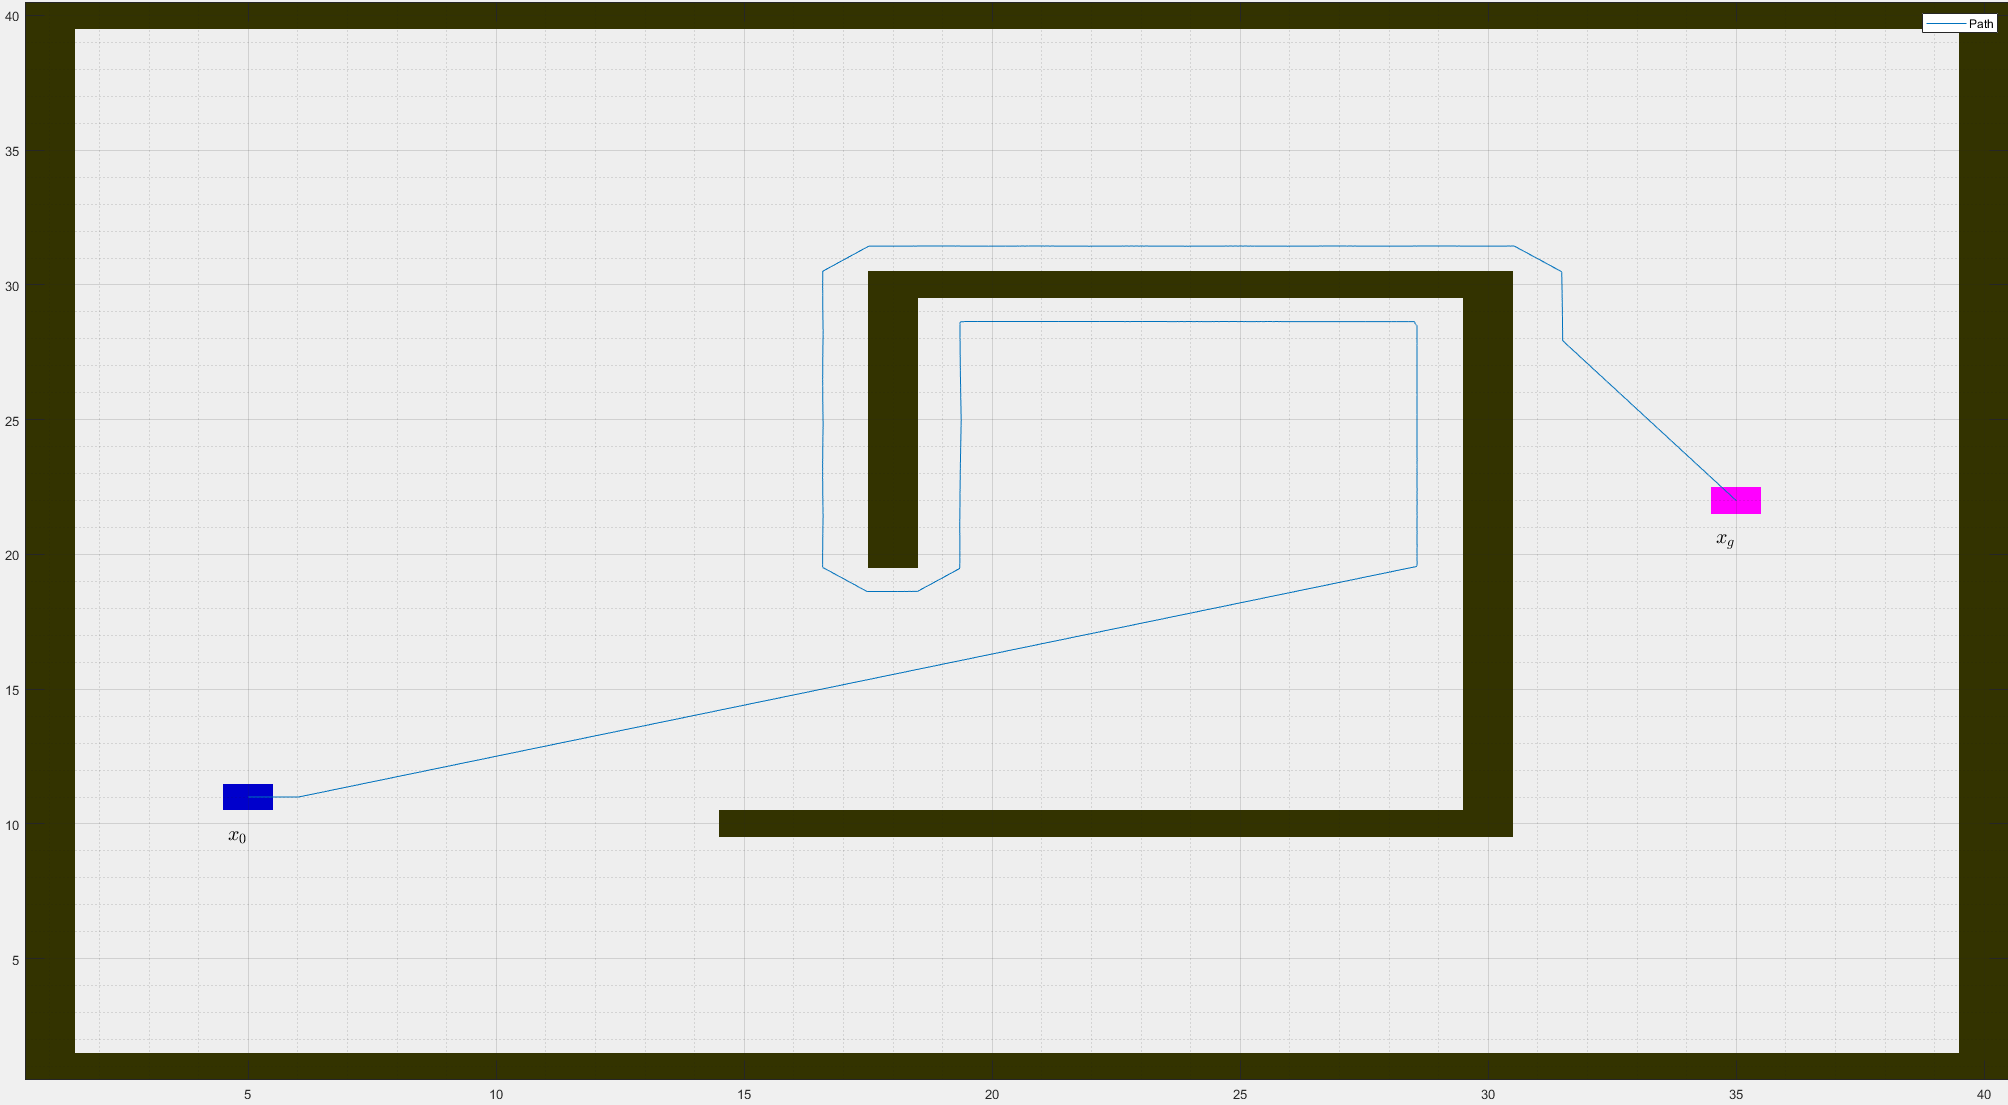
\includegraphics[width=\columnwidth]{images/robot_path.png}
    \caption{Trajectory of the robot through the maze.}
    \label{fig:robot_path}
\end{figure}

%======================================================================================
% Present three subplots

The subplot shown in Fig.\:\ref{fig:x_time} shows x of the robot as a function of time. In subplot Fig.\:\ref{fig:y_time} the same is shown but for y. $\theta_{\text{ref}}$ compared to $\theta$ with respect to time is shown in Fig.\:\ref{fig:theta_time}. The heavy clipping occuring in Fig.\:\ref{fig:theta_time} is the result of constraining all angles to $[-\pi, \pi]$, therefor angles close to $-\pi$ or $\pi$ can jump between the two when incremented or decremented slightly.
\begin{figure}
	\centering
    \begin{subfigure}[t]{0.32\columnwidth}
		\centering
		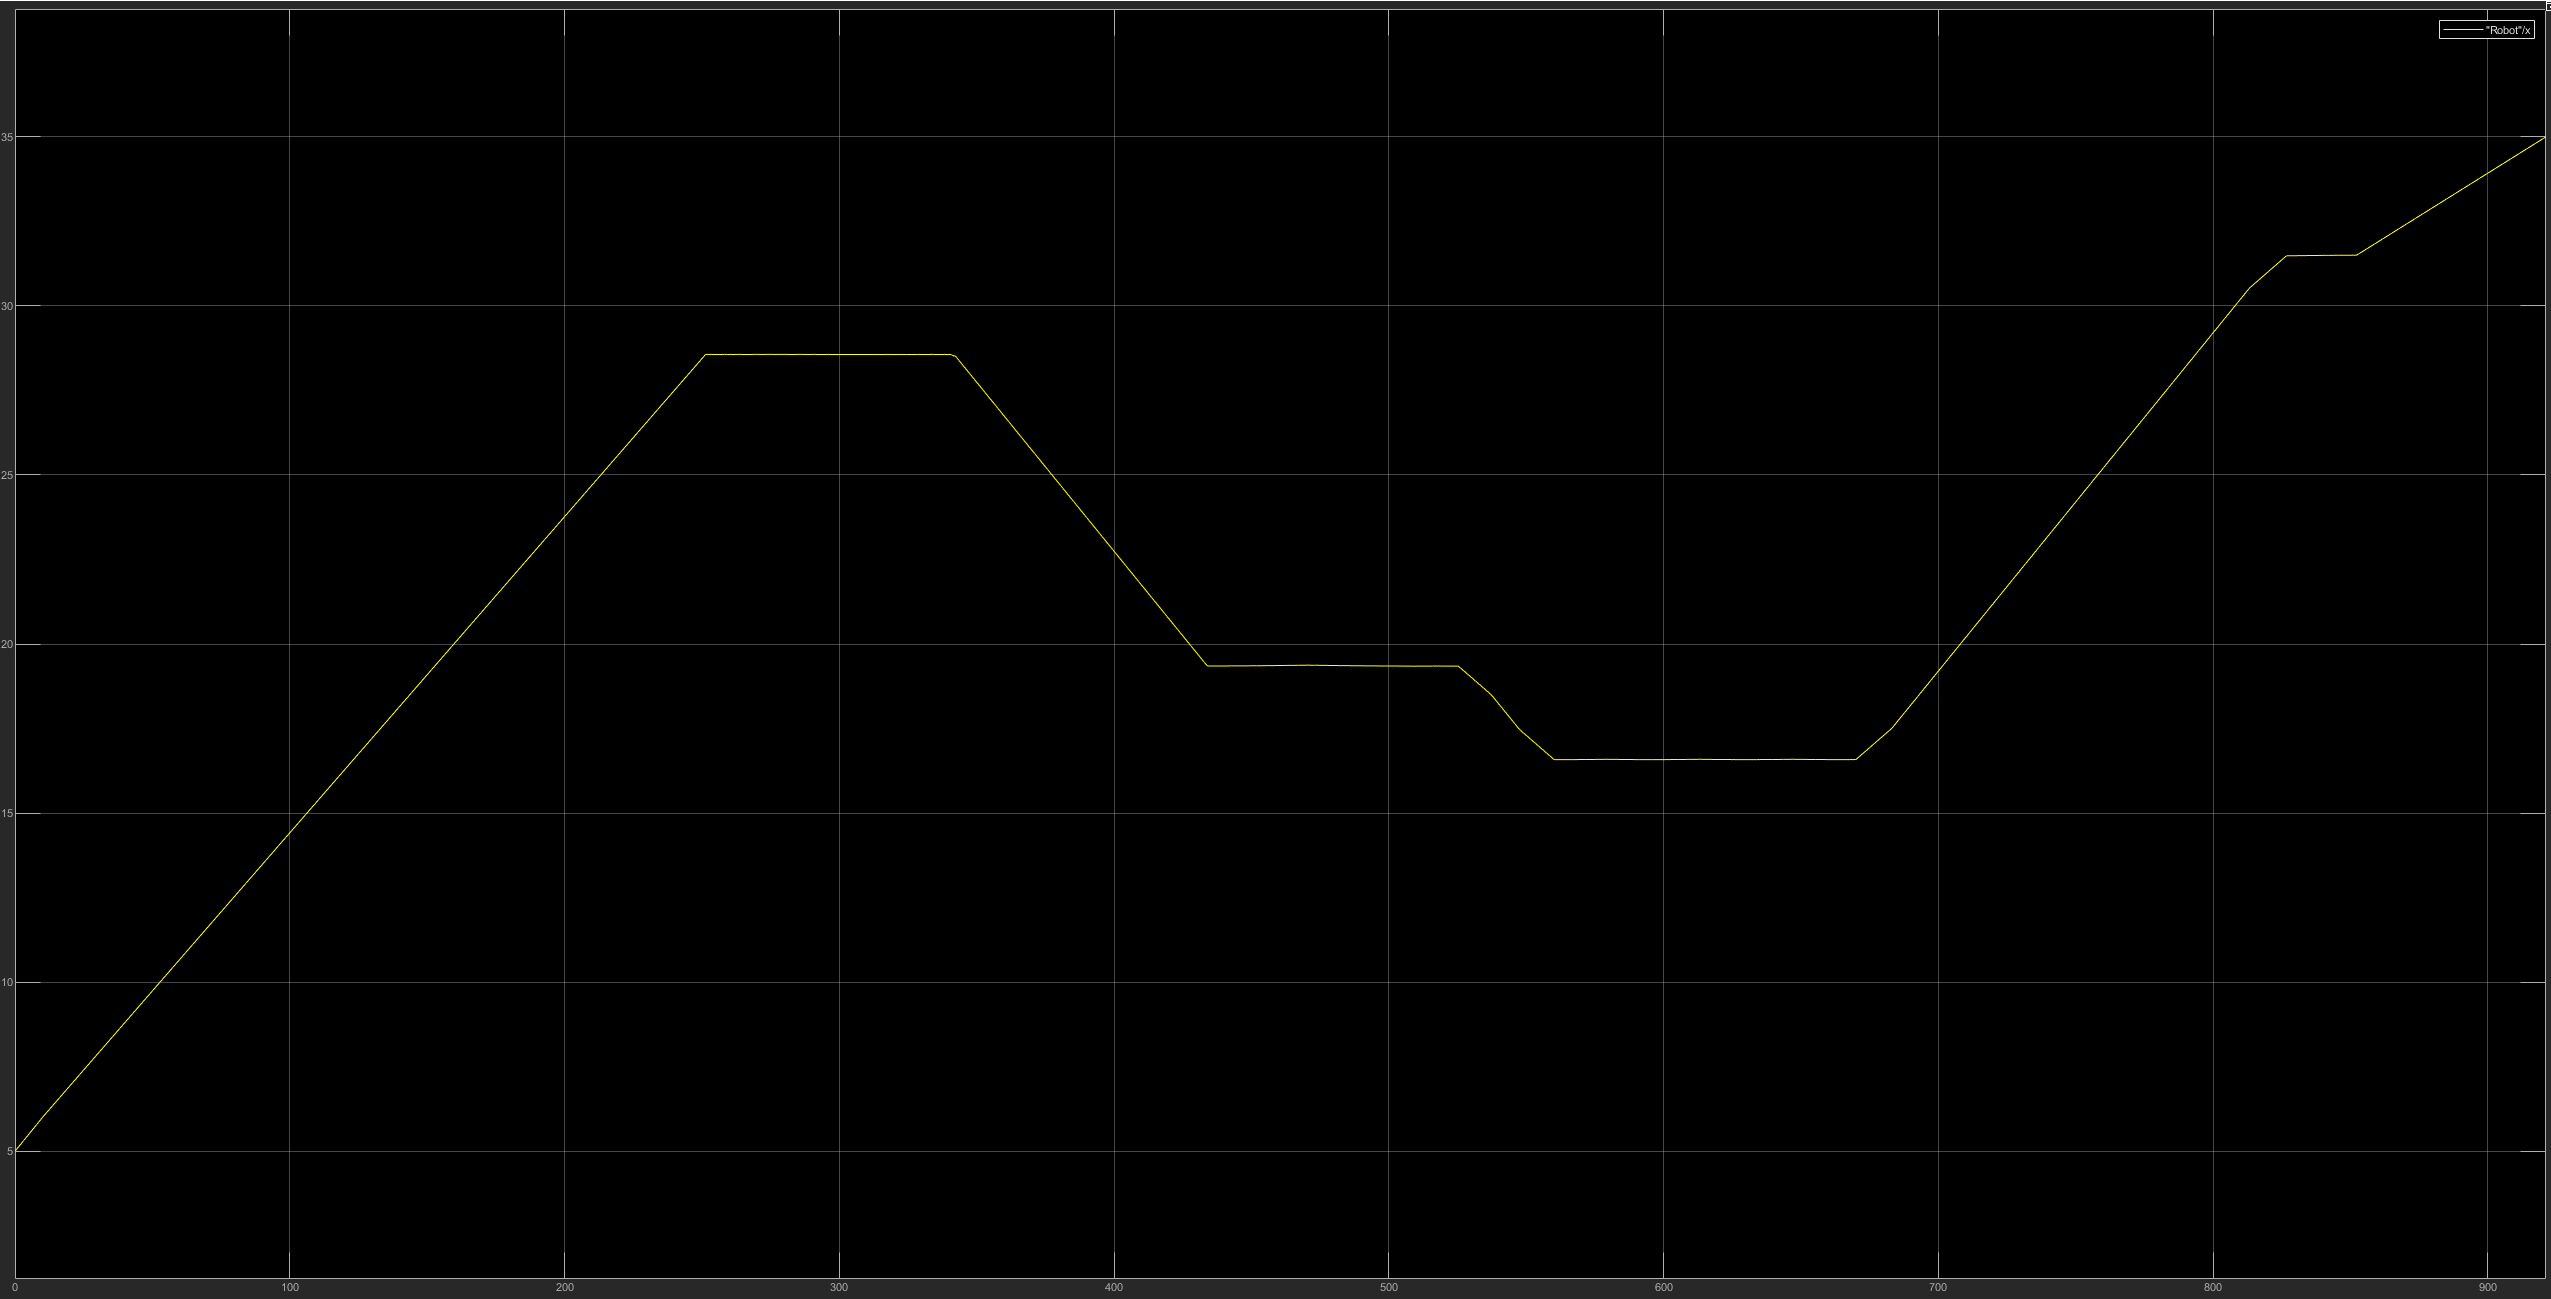
\includegraphics[width=\textwidth]{images/x_time.png}
		\caption{x coordinate of the robot as a function of time.}
        \label{fig:x_time}
	\end{subfigure}
    \hfill
	\begin{subfigure}[t]{0.32\columnwidth}
		\centering
		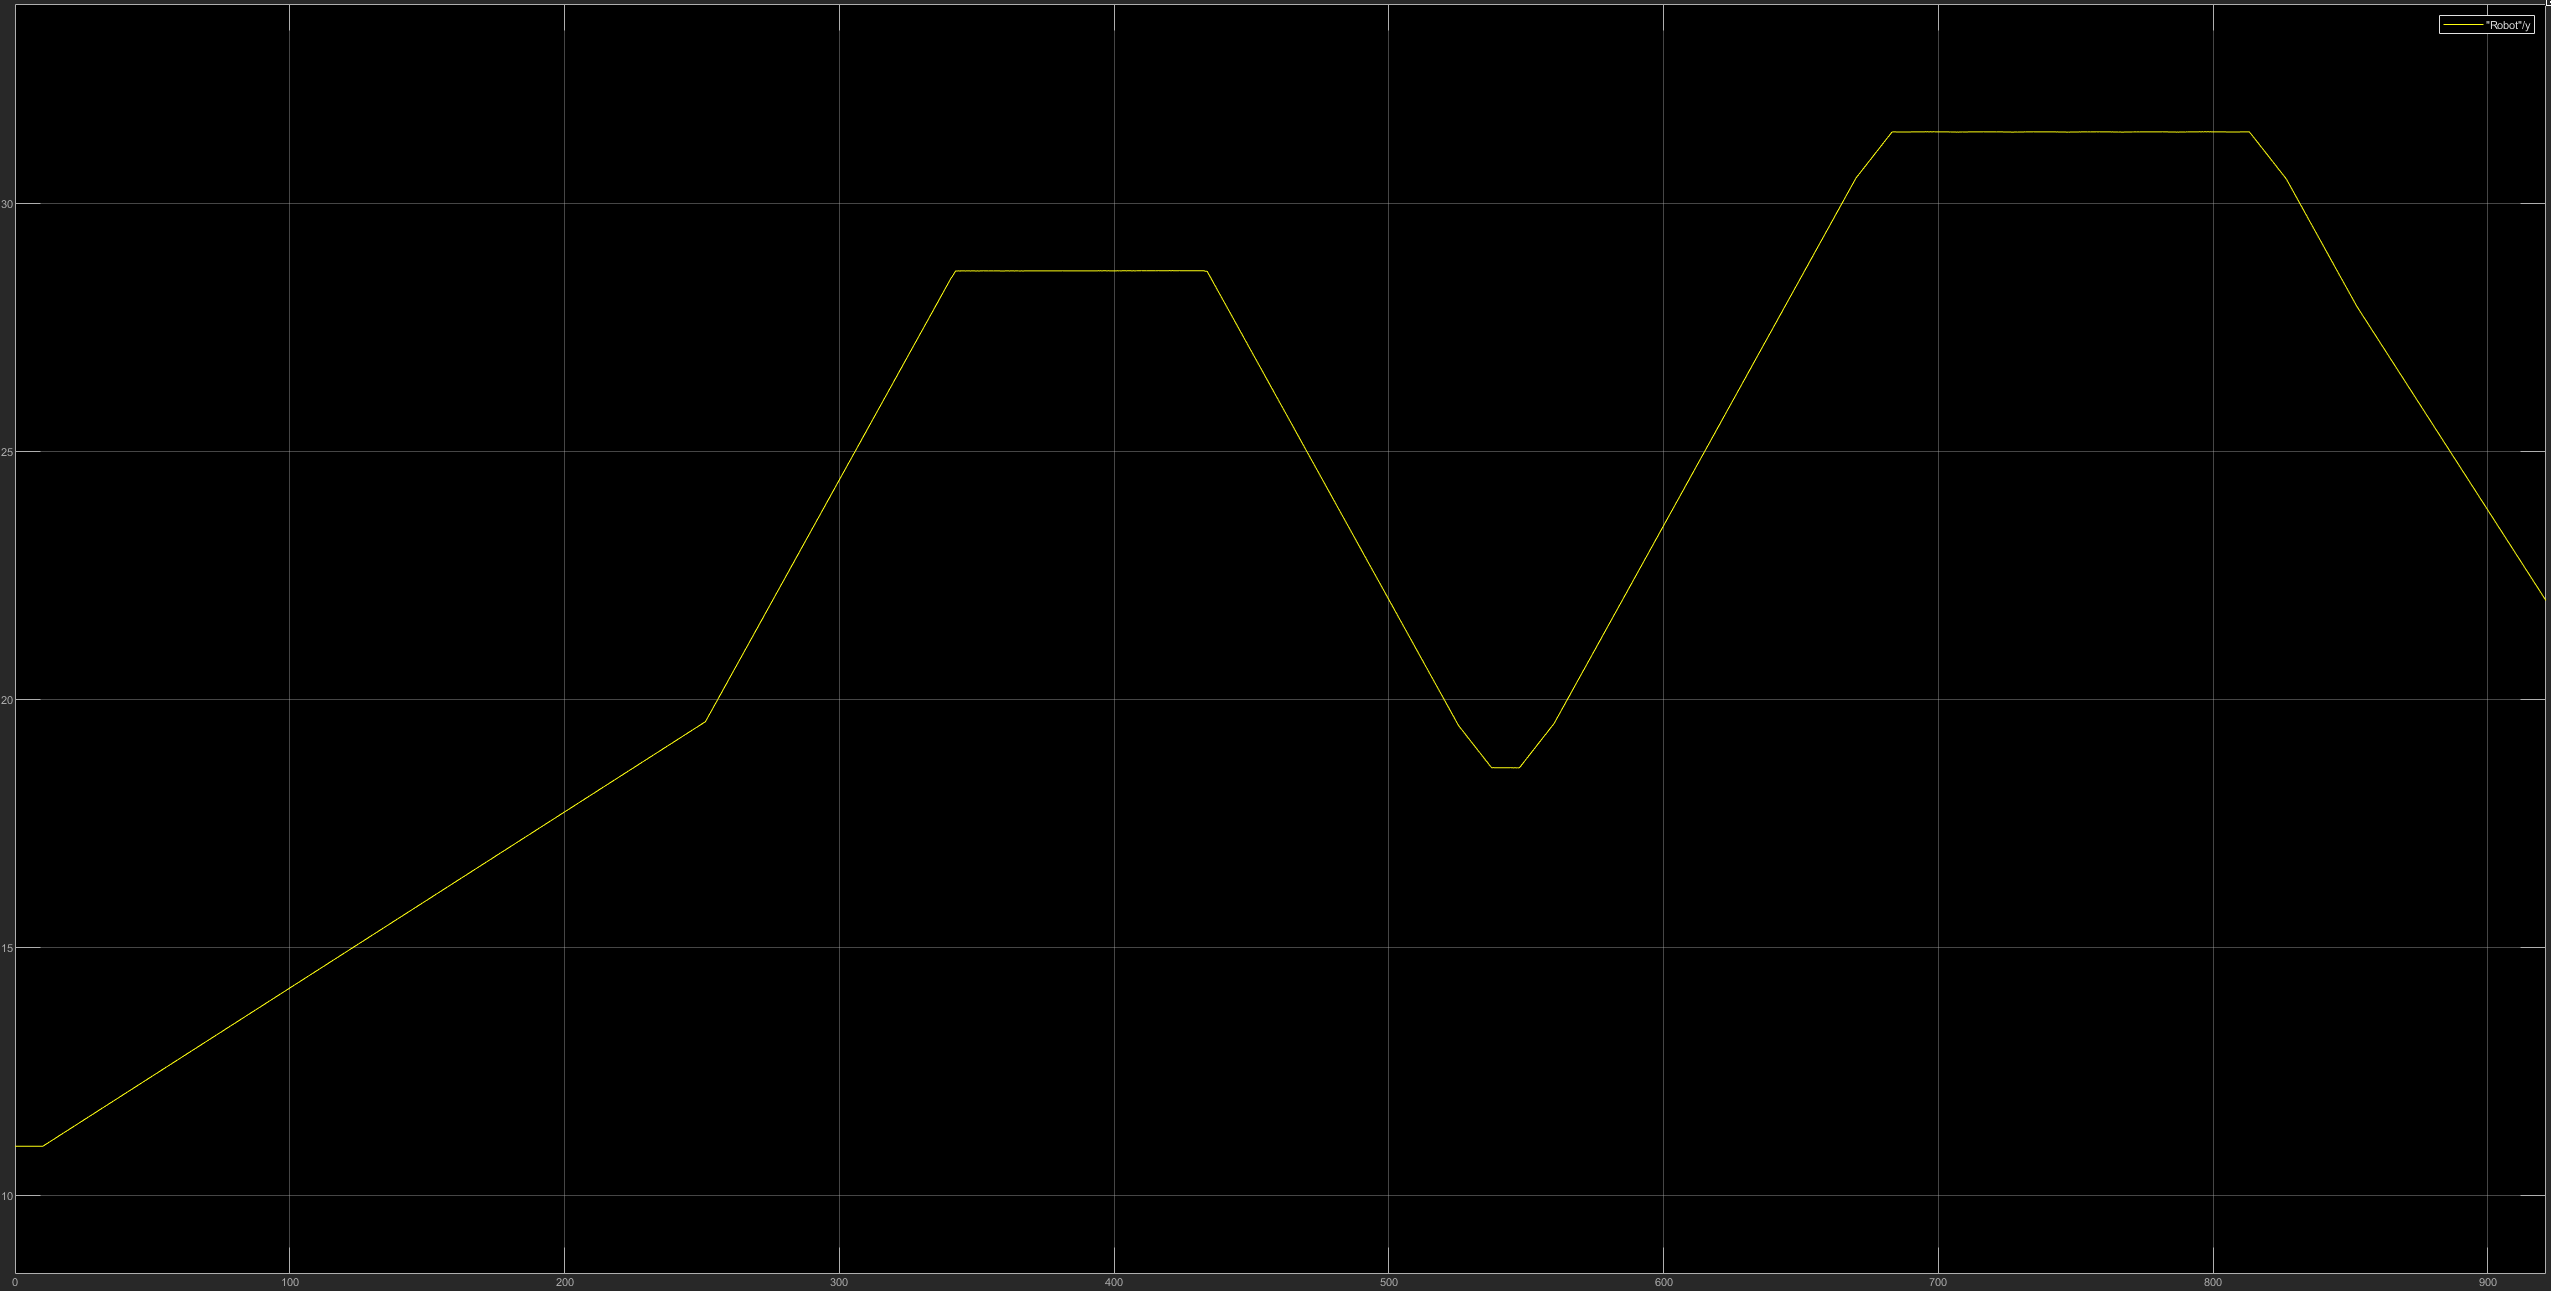
\includegraphics[width=\textwidth]{images/y_time.png}
		\caption{y coordinate of the robot as a function of time.}
        \label{fig:y_time}
	\end{subfigure}
    \hfill
    \begin{subfigure}[t]{0.32\columnwidth}
		\centering
		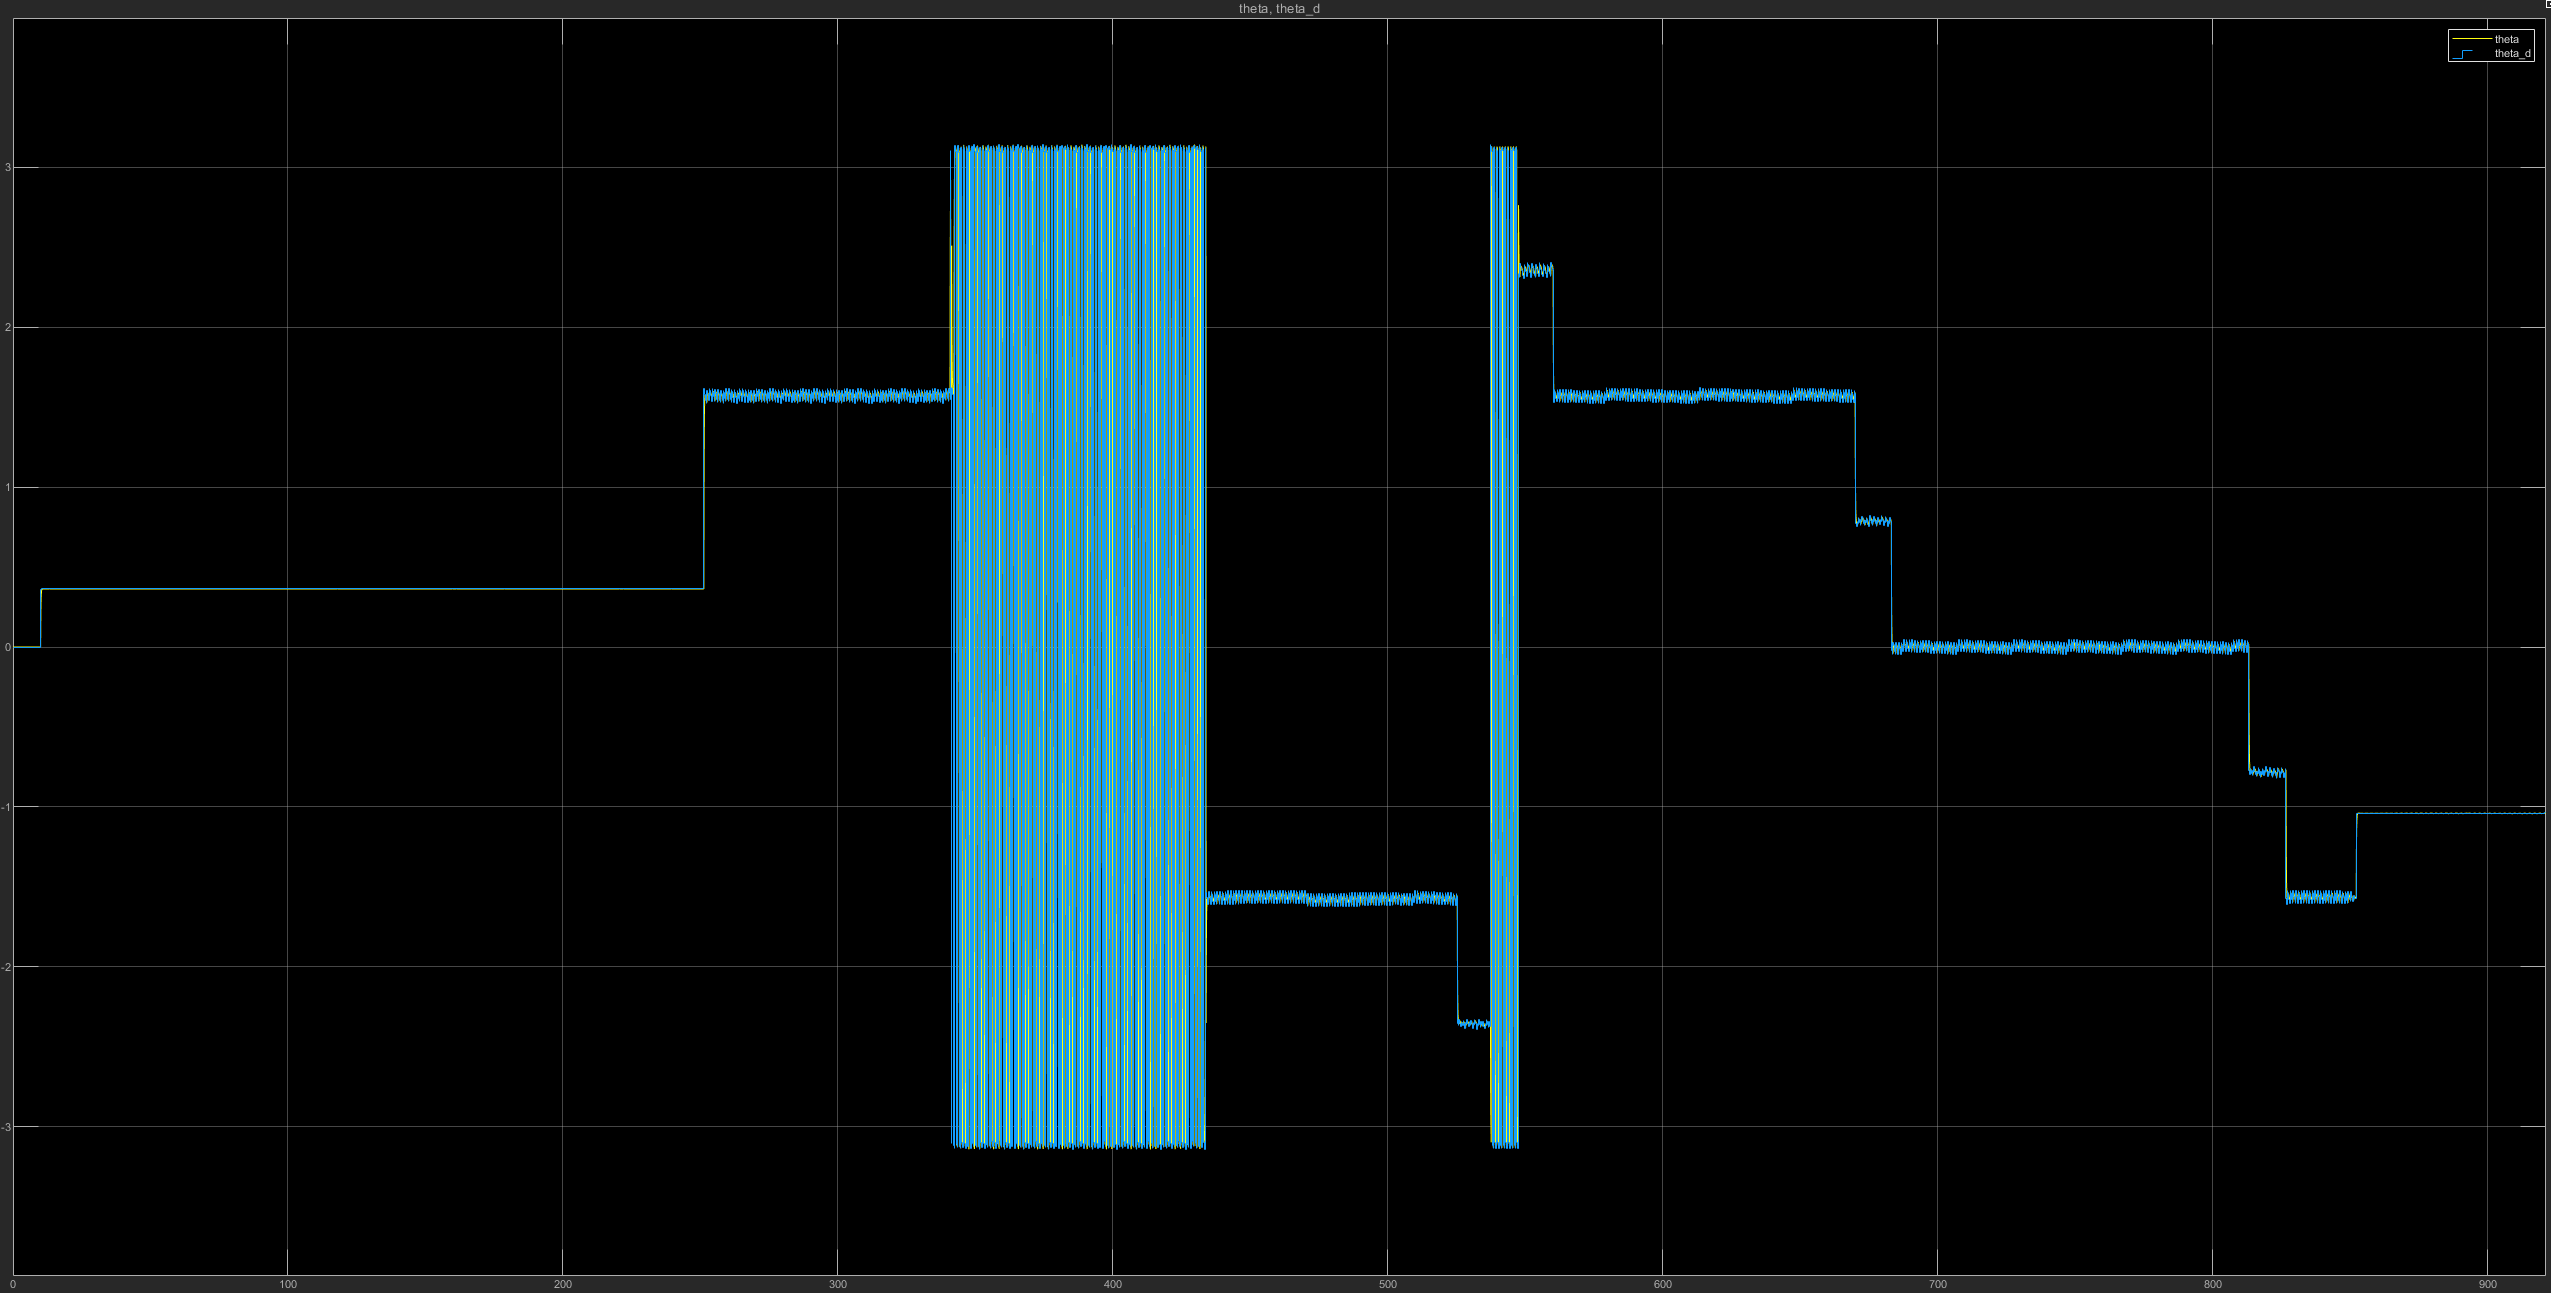
\includegraphics[width=\textwidth]{images/theta_time.png}
		\caption{$\theta_{\text{ref}}$ ($\theta_{\text{desired}}$) compared to $\theta$ of the robot as a function of time.}
        \label{fig:theta_time}
	\end{subfigure}
	\caption{Robot pose as functions of time.}
    \label{fig:x_y_theta_sub}
\end{figure}

%======================================================================================


%======================================================================================
\begin{comment}
    
\end{comment}
%======================================================================================
\section{Discussion}
%======================================================================================

The system could be implemented on a physical platform in real life, however there are many considerations which needs to be take in to account, some notable ones will be covered in this section.

% Real world implementation differences
The simulated systems level of discretization is unrealistic for real world scenarios, the system would have to go through extensive testing and most likely multiple revisions to ensure the system functions correctly for the continuous nature of the real world.
The current model also has no simulated noise. Sensor noise and inaccuracies will most definitely have to be dealt with adequately in a real world implementation.
Depending on the expected deployment area, factors such as weather, lighting and other dynamic environmental factors are not covered in the model and the system would have to be modified to handle such dynamic effects.
Physical limitations and constraints were not considered in the simulated model. This includes such things as: actuator limits, friction and wear.
In real world scenarios the wheels can loose contact with the ground or slippage causing unaccounted action to take place which will cause errors in the pose estimation.
It should be noted that implementation of this system in real life would require a priori information about the environment since the current structure of the system requires knowledge about the goal location.

% Possible sensor choices
Possible sensors for this system would be a LIDAR as the sensor for identifying distance and angles to obstacles, and an inertial measurement unit (IMU) containing an accelerometer, a gyroscope and a magnetometer in the same package (called IMMU), for approximating the robots current pose (position and orientation). It should be noted that this setup is subject to drift and error accumulation. If the system was to only be employed in outside environments, then a GPS could be implemented as well to help negate error accumulation of the robot pose estimation, stemming from the IMMU, and help to better approximate the current pose.

% Sensor noise
Sensor noise is a severe problem, one way to mitigate it is to use sensor fusion, this could be done by employing a Kalman filter. A Kalman filter can also be used to filter the signal and thus reducing sensor noise, particle filters are also viable for this.
Better sensors would naturally also reduce the issue of sensor noise but will significantly increase cost which often is a limiting factor.

% Problems with behavior robotics in other environments
The system could encounter various problems depending on the environment. The sensors proposed for calculating position and orientation, IMMU and GPS, severely limit the possible environments. GPS mainly works in outdoor environments, and both IMMU and GPS would work poorly in underwater applications. 
The behavior robotics in the system works well for the simulated environment but could pose various challenges in dynamic environments, especially containing human interaction.
While the behavior robotics works sufficiently well for the complexity of the simulated map, it might struggle with more complex environments.
The behavior is also static, containing no capabilities of learning. While this might be sufficient for simple problems, it might cause problems in more difficult scenarios, especially if one considers limitations of resources like time or energy. The reason for this is that while the static behavior might solve a more difficult problem, this solution might be far from the global optimal or even from a local optimal, and it will never improve. If the system then also has limited resources like time or energy, then it is easy to see that a more sophisticate system is required which is guaranteed to find a more optimal solution within the constraints of available resources.

%======================================================================================


%======================================================================================
\begin{comment}
    % Discuss how you approached the design of different behaviors and the values chosen for control parameters. Reflect on potential real-world implementation differences, sensor noise, sensor choices, and possible issues in behavior robotics for varied environments.
    % Expand the report to include some reflection about how the system could be implemented on a physical platform and what would differ from the simulation. For example, how could the robot deal with sensor noise? What kind of sensors could be used? Can you spot any potential problems with behavior robotics for other environments?
\end{comment}
%======================================================================================
%\section{Conclusion}
%======================================================================================

%======================================================================================


%======================================================================================
\begin{comment}
    % Summarize the findings, learned lessons, and potential areas for future work.
\end{comment}
%======================================================================================
\appendix
%======================================================================================

%\section{Code}

%======================================================================================

\begin{comment}

\section{Mapping between frames}
The mapping of a robot position $\mathbf{p}_i$ (in operational space), from the frame attached to the robot, denoted $2$, to the base frame, denoted $1$, assuming only rotation and no translation between the frames, follow\:\eqref{eq:map_position_rotation}. 

\begin{dmath}
    \label{eq:map_position_rotation}
    \mathbf{p}_1 = \mathbf{R}_{\text{z}}(\theta) \mathbf{p}_2
\end{dmath}
Here it is assumed that the rotation between the two frames are about the z axis by an angle $\theta$.

If the frames contain translation and rotation, then the use of homogeneous matrices ($\mathbf{A}_i^{i-1}$) needs to be employed following the Denavit–Hartenberg convention, see\:\eqref{eq:map_position_homogenous}.

\begin{dmath}
    \label{eq:map_position_homogenous}
    \begin{bmatrix}
    \mathbf{p}_1 \\
    1
    \end{bmatrix}
    = \mathbf{A}_2^1 
    \begin{bmatrix}
    \mathbf{p}_2 \\
    1
    \end{bmatrix}
\end{dmath}

Where $\mathbf{A}$ is in the form of\:\eqref{eq:homogenous_matrix}.

\begin{dmath}
    \label{eq:homogenous_matrix}
    \mathbf{A} = 
    \begin{bmatrix}
    \mathbf{R} & \mathbf{p} \\
    0 & 1
    \end{bmatrix}
\end{dmath}

\end{comment}

%======================================================================================


%======================================================================================
\begin{comment}
    % Include or reference your script and Simulink model.
\end{comment}
%======================================================================================

% Include refs
\bibliographystyle{IEEEtran}
\bibliography{refs}

\end{document}
%======================================================================================